\documentclass[11pt]{beamer}
\usepackage[utf8]{inputenc}
\usepackage[T1]{fontenc}
\usepackage{lmodern}
\usepackage[english]{babel}
\usepackage{graphicx}
\usepackage[most]{tcolorbox}
\usetheme{Darmstadt}
\setbeamertemplate{navigation symbols}{}
\setbeamertemplate{footline}{
	\begin{beamercolorbox}[ht=3ex,leftskip=1.4cm,rightskip=.3cm]{author in head/foot}
		\hfill \insertframenumber
		\vspace*{0.07cm}
	\end{beamercolorbox}
} 
\usepackage{url}
\usepackage{hyperref}
\usepackage{listings}
\usepackage{upquote}
\usepackage{amsmath}
\usepackage{booktabs}

% color def
\usepackage{color}
\definecolor{darkred}{rgb}{0.6,0.0,0.0}
\definecolor{darkgreen}{rgb}{0,0.50,0}
\definecolor{lightblue}{rgb}{0.0,0.42,0.91}
\definecolor{orange}{rgb}{0.99,0.48,0.13}
\definecolor{grass}{rgb}{0.18,0.80,0.18}
\definecolor{pink}{rgb}{0.97,0.15,0.45}

\usepackage{nth}

% General Setting of listings
\lstset{
	language=Python,
	tabsize=4,
	aboveskip=1em,
	breaklines=true,
	abovecaptionskip=-6pt,
	captionpos=b,
	escapeinside={\%*}{*)},
	frame=single,
	numbers=left,
	numbersep=8pt,
	numberstyle=\tiny,
	morekeywords=[1]{,as,assert,nonlocal,with,yield,self,True,False,None,} % Python builtin
	morekeywords=[2]{,__init__,__add__,__mul__,__div__,__sub__,__call__,__getitem__,__setitem__,__eq__,__ne__,__nonzero__,__rmul__,__radd__,__repr__,__str__,__get__,__truediv__,__pow__,__name__,__future__,__all__,}, % magic methods
	morekeywords=[3]{,object,type,isinstance,copy,deepcopy,zip,enumerate,reversed,list,set,len,dict,tuple,range,xrange,append,execfile,real,imag,reduce,str,repr,}, % common functions
	morekeywords=[4]{,Exception,NameError,IndexError,SyntaxError,TypeError,ValueError,OverflowError,ZeroDivisionError,}, % errors
	morekeywords=[5]{,ode,fsolve,sqrt,exp,sin,cos,arctan,arctan2,arccos,pi, array,norm,solve,dot,arange,isscalar,max,sum,flatten,shape,reshape,find,any,all,abs,plot,linspace,legend,quad,polyval,polyfit,hstack,concatenate,vstack,column_stack,empty,zeros,ones,rand,vander,grid,pcolor,eig,eigs,eigvals,svd,qr,tan,det,logspace,roll,min,mean,cumsum,cumprod,diff,vectorize,lstsq,cla,eye,xlabel,ylabel,squeeze,}, % numpy / math
	deletekeywords=[2]{next,set},
	deletekeywords=[3]{next,set},
	basicstyle=\ttfamily\small,
	backgroundcolor=\color{white},
	commentstyle=\color{darkgreen}\slshape,
	keywordstyle=\color{blue}\bfseries\itshape,
	keywordstyle=[2]\color{blue}\bfseries,
	keywordstyle=[3]\color{grass},
	keywordstyle=[4]\color{red},
	keywordstyle=[5]\color{orange},
	stringstyle=\color{darkred},
	emphstyle=\color{pink}\underbar,
	morestring=*[d]{"},
}

\usepackage{tikz}
\usetikzlibrary{calc,shapes.multipart,chains,arrows,positioning,overlay-beamer-styles,arrows.meta,bending}

\tikzset{  
    vertex/.style={circle, draw, minimum size=8mm, thick},
    edge/.style={draw, -{Stealth[length=3mm]}},
    biedge/.style={draw, {Stealth[length=3mm]}-{Stealth[length=3mm]}},
    weight/.style={midway, fill=white, inner sep=1pt}
}


\begin{document}
	\author{Data Structures}
	\title{Graphs}
	\titlegraphic{
\includegraphics[width=3cm]{img/UPNA}}
	\date[]{2024-2025}
	\subject{Data Structures}
	%\subtitle{}
	%\logo{}
	%\institute{}
	%\date{}
	%\subject{}
	%\setbeamercovered{transparent}
	%\setbeamertemplate{navigation symbols}{}
	\begin{frame}[plain]
		\maketitle
	\end{frame}

	\begin{frame}
		\tableofcontents
	\end{frame}

\section{What is a Graph?}

\begin{frame}\frametitle{What is a Graph?}
\begin{itemize}
\item How can google maps find the path from a city to another?
\item How does facebook, twitter... keep track of relations between users?
\item If we try to represent the Internet as a drawing what shape will it have?
\end{itemize}
\end{frame}

\begin{frame}\frametitle{Definition}
\begin{itemize}
\item A graph is a structure that represents relationships between elements
\item A tuple of vertices and edges
\begin{itemize}
    \item A set of vertices: $V = {v_1, v_2, ..., v_n}$
    \item A set of edges: $E = {e_1, e_2, ..., e_m}$
\end{itemize}
\pause
\hspace{1cm}
\begin{block}{}
$$
G = (V, E)
$$
\end{block}
\end{itemize}
\end{frame}

\subsection{Basic Terminology}

\begin{frame}\frametitle{Vertex}
\begin{itemize}
\item Also known as nodes
\end{itemize}
\begin{center}
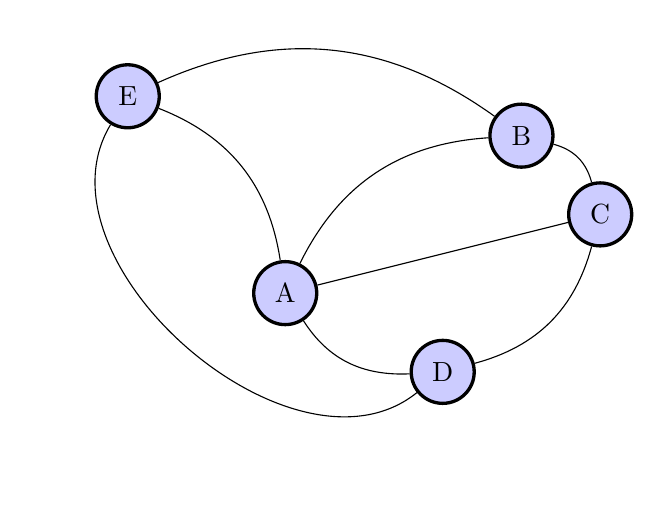
\begin{tikzpicture}[scale=1, transform shape]
    % Nodes
    \node[vertex, very thick, fill=blue!20] (A) at (0,0) {A};
    \node[vertex, very thick, fill=blue!20] (B) at (3,2) {B};
    \node[vertex, very thick, fill=blue!20] (C) at (4,1) {C};
    \node[vertex, very thick, fill=blue!20] (D) at (2,-1) {D};
    \node[vertex, very thick, fill=blue!20] (E) at (-2, 2.5) {E};

    % edges
    \draw (A) to[bend left] (B);
    \draw (B) to[bend left] (C);
    \draw (C) to[bend left] (D);
    \draw (D) to[bend left] (A);
    \draw (A) -- (C); 
    \draw (E) to[bend right=80] (D);
    \draw (E) to[bend left] (B);
    \draw (E) to[bend left] (A);
\end{tikzpicture}
\end{center}
\end{frame}

\begin{frame}\frametitle{Edge}
\begin{center}
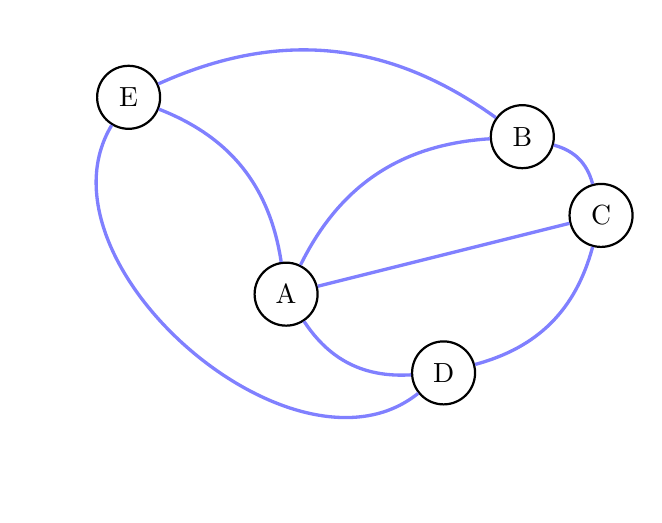
\begin{tikzpicture}[scale=1, transform shape]
    % Nodes
    \node[vertex] (A) at (0,0) {A};
    \node[vertex] (B) at (3,2) {B};
    \node[vertex] (C) at (4,1) {C};
    \node[vertex] (D) at (2,-1) {D};
    \node[vertex] (E) at (-2, 2.5) {E};

    % edges
    \draw[very thick, color=blue!50] (A) to[bend left] (B);
    \draw[very thick, color=blue!50] (B) to[bend left] (C);
    \draw[very thick, color=blue!50] (C) to[bend left] (D);
    \draw[very thick, color=blue!50] (D) to[bend left] (A);
    \draw[very thick, color=blue!50] (A) -- (C); 
    \draw[very thick, color=blue!50] (E) to[bend right=80] (D);
    \draw[very thick, color=blue!50] (E) to[bend left] (B);
    \draw[very thick, color=blue!50] (E) to[bend left] (A);
\end{tikzpicture}
\end{center}
\end{frame}


\begin{frame}\frametitle{Path}
\begin{itemize}
\item A sequence of edges that connect vertices
\end{itemize}
\begin{center}
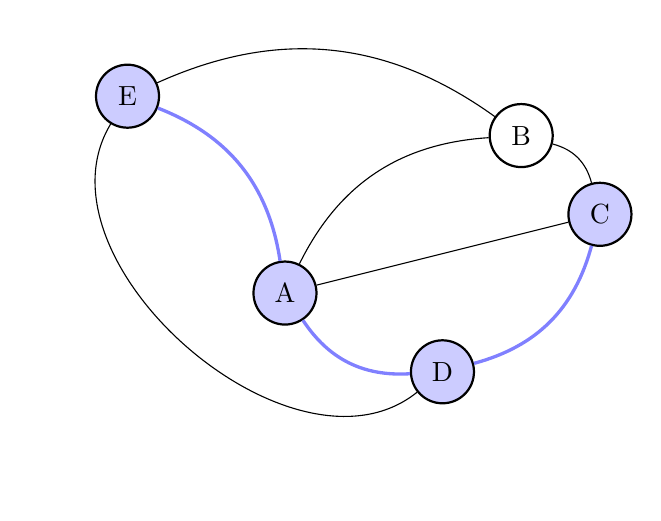
\begin{tikzpicture}[scale=1, transform shape]
    % Nodes
    \node[vertex, fill=blue!20] (A) at (0,0) {A};
    \node[vertex] (B) at (3,2) {B};
    \node[vertex, fill=blue!20] (C) at (4,1) {C};
    \node[vertex, fill=blue!20] (D) at (2,-1) {D};
    \node[vertex, fill=blue!20] (E) at (-2, 2.5) {E};

    % edges
    \draw (A) to[bend left] (B);
    \draw (B) to[bend left] (C);
    \draw[very thick, color=blue!50] (C) to[bend left] (D);
    \draw[very thick, color=blue!50] (D) to[bend left] (A);
    \draw (A) -- (C); 
    \draw (E) to[bend right=80] (D);
    \draw (E) to[bend left] (B);
    \draw[very thick, color=blue!50] (E) to[bend left] (A);
\end{tikzpicture}
\end{center}
\end{frame}


\begin{frame}\frametitle{Connection Between Elements}
\begin{block}{}
Is the following a graph? % YES
\end{block}
\begin{center}
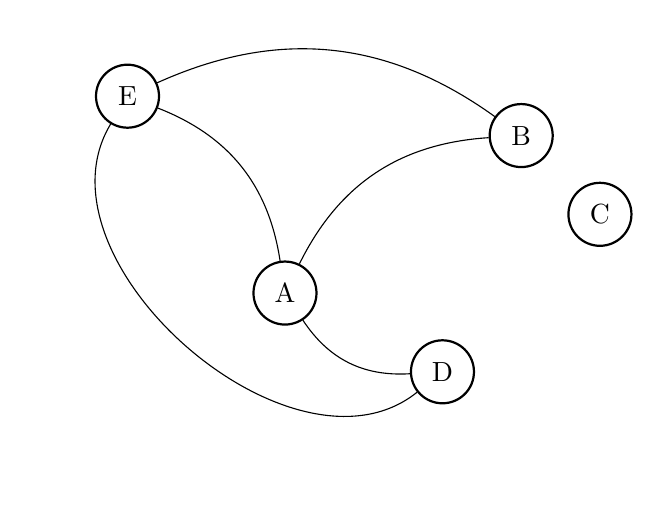
\begin{tikzpicture}[scale=1, transform shape]
    % Nodes
    \node[vertex] (A) at (0,0) {A};
    \node[vertex] (B) at (3,2) {B};
    \node[vertex] (C) at (4,1) {C};
    \node[vertex] (D) at (2,-1) {D};
    \node[vertex] (E) at (-2, 2.5) {E};

    % edges
    \draw (A) to[bend left] (B);
    %\draw (B) to[bend left] (C);
    %\draw (C) to[bend left] (D);
    \draw (D) to[bend left] (A);
    %\draw (A) -- (C); 
    \draw (E) to[bend right=80] (D);
    \draw (E) to[bend left] (B);
    \draw (E) to[bend left] (A);
\end{tikzpicture}
\end{center}
\end{frame}

\begin{frame}\frametitle{Self Edges}
\begin{itemize}
\item Some graphs allow self edges
\end{itemize}
\begin{center}
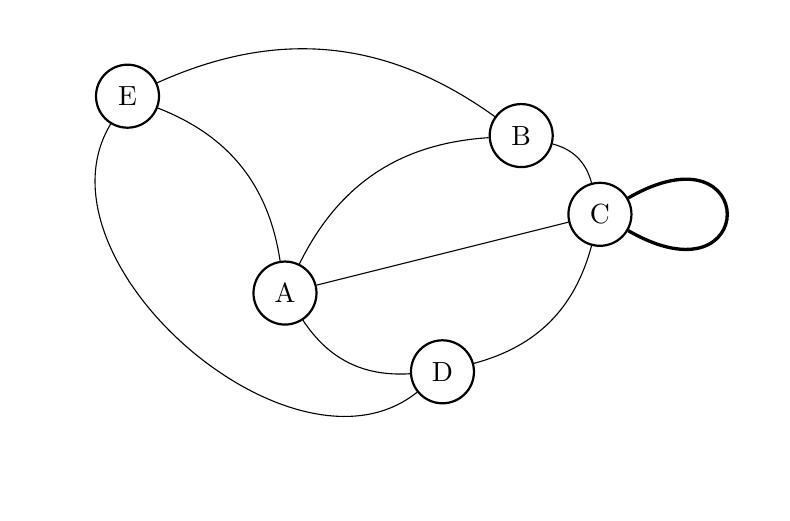
\begin{tikzpicture}[scale=1, transform shape]
    % Nodes
    \node[vertex] (A) at (0,0) {A};
    \node[vertex] (B) at (3,2) {B};
    \node[vertex] (C) at (4,1) {C};
    \node[vertex] (D) at (2,-1) {D};
    \node[vertex] (E) at (-2, 2.5) {E};

    % edges
    \draw (A) to[bend left] (B);
    \draw (B) to[bend left] (C);
    \draw (C) to[bend left] (D);
    \draw (D) to[bend left] (A);
    \draw (A) -- (C); 
    \draw (E) to[bend right=80] (D);
    \draw (E) to[bend left] (B);
    \draw (E) to[bend left] (A);
    \draw[very thick] (C) to[in=-30, out=30, looseness=12] (C);
\end{tikzpicture}
\end{center}
\end{frame}

\section{Types of Graphs}

\subsection{Undirected}

\begin{frame}\frametitle{Undirected Graphs}
\begin{itemize}
\item Edges have no specific direction
    \begin{itemize}
    \item Edges will always be bidirectional
    \item The edge ${A,B}$ is the same as ${B,A}$
    \end{itemize}
\pause
\item What could be a real life example of an undirected graph? % facebook friends
%\item $G=(V,E)$ where:
%    \begin{itemize}
%    \item \( E \subseteq \{ \{u, v\} \mid u, v \in V, u \neq v \} \) is the set of edges
%    \end{itemize}
\end{itemize}
\end{frame}

\begin{frame}\frametitle{Degree}
\begin{itemize}
\item Number of edges connected to a vertex
\end{itemize}
\begin{center}
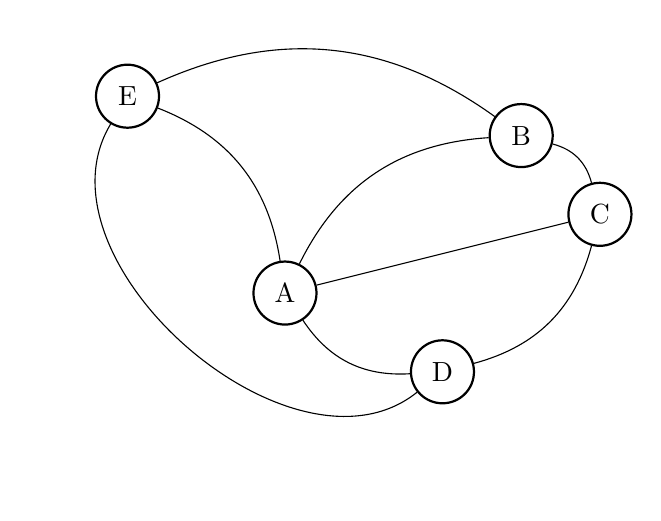
\begin{tikzpicture}[scale=1, transform shape]
    % Nodes
    \node[vertex] (A) at (0,0) {A};
    \node[vertex] (B) at (3,2) {B};
    \node[vertex] (C) at (4,1) {C};
    \node[vertex] (D) at (2,-1) {D};
    \node[vertex] (E) at (-2, 2.5) {E};

    % edges
    \draw (A) to[bend left] (B);
    \draw (B) to[bend left] (C);
    \draw (C) to[bend left] (D);
    \draw (D) to[bend left] (A);
    \draw (A) -- (C); 
    \draw (E) to[bend right=80] (D);
    \draw (E) to[bend left] (B);
    \draw (E) to[bend left] (A);
\end{tikzpicture}
\end{center}
\end{frame}

\begin{frame}\frametitle{Degree}
\begin{itemize}
\item Number of edges connected to a vertex
\end{itemize}
\begin{center}
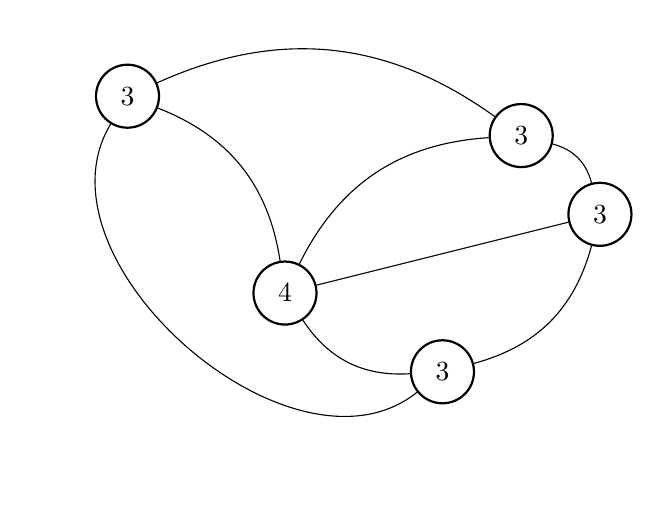
\begin{tikzpicture}[scale=1, transform shape]
    % Nodes
    \node[vertex] (A) at (0,0) {4};
    \node[vertex] (B) at (3,2) {3};
    \node[vertex] (C) at (4,1) {3};
    \node[vertex] (D) at (2,-1) {3};
    \node[vertex] (E) at (-2, 2.5) {3};

    % edges
    \draw (A) to[bend left] (B);
    \draw (B) to[bend left] (C);
    \draw (C) to[bend left] (D);
    \draw (D) to[bend left] (A);
    \draw (A) -- (C); 
    \draw (E) to[bend right=80] (D);
    \draw (E) to[bend left] (B);
    \draw (E) to[bend left] (A);
\end{tikzpicture}
\end{center}
\end{frame}

\subsection{Directed}

\begin{frame}\frametitle{Directed Graphs}
\begin{itemize}
\item Edges can have direction
\item Each edge will have a source and a destination
\end{itemize}
\begin{center}
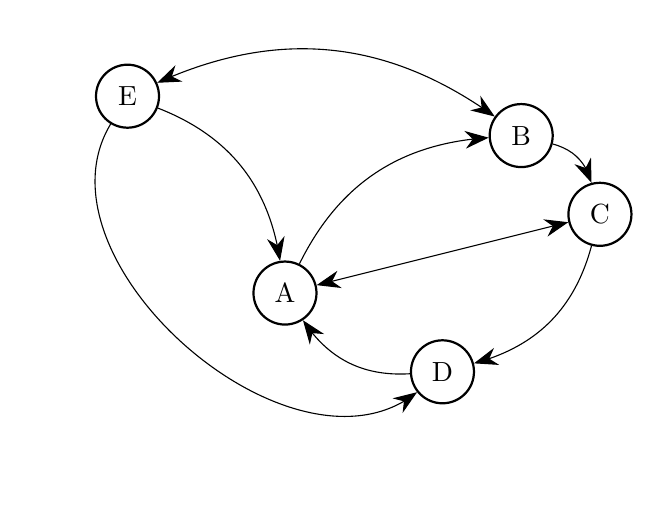
\begin{tikzpicture}[scale=1, transform shape]
    % Nodes
    \node[vertex] (A) at (0,0) {A};
    \node[vertex] (B) at (3,2) {B};
    \node[vertex] (C) at (4,1) {C};
    \node[vertex] (D) at (2,-1) {D};
    \node[vertex] (E) at (-2, 2.5) {E};

    % edges
    \draw[edge] (A) to[bend left] (B);
    \draw[edge] (B) to[bend left] (C);
    \draw[edge] (C) to[bend left] (D);
    \draw[edge] (D) to[bend left] (A);
    \draw[biedge] (A) -- (C); 
    \draw[edge] (E) to[bend right=80] (D);
    \draw[biedge] (E) to[bend left] (B);
    \draw[edge] (E) to[bend left] (A);
\end{tikzpicture}
\end{center}
\end{frame}

\begin{frame}\frametitle{Degree}
\begin{itemize}
\item We can differentiate two degrees for a vertex
    \begin{description}
        \item[In-degree:] The number of incoming edges
        \item[Out-degree:] The number of outgoing edges
    \end{description}
\end{itemize}
\end{frame}

\begin{frame}\frametitle{In-degree}
\begin{center}
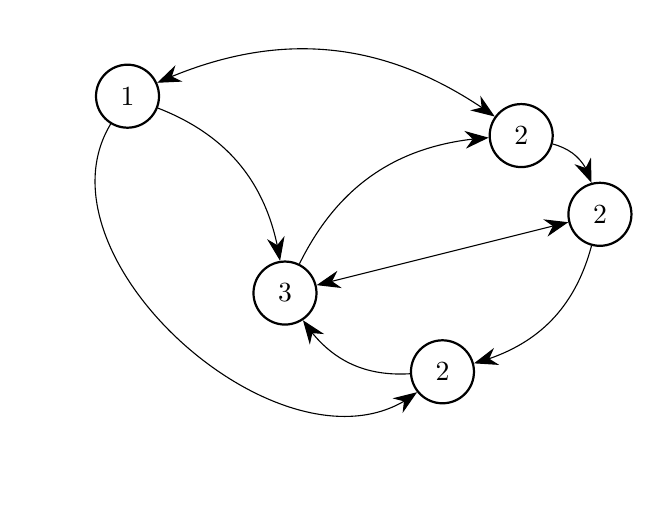
\begin{tikzpicture}[scale=1, transform shape]
    % Nodes
    \node[vertex] (A) at (0,0) {3};
    \node[vertex] (B) at (3,2) {2};
    \node[vertex] (C) at (4,1) {2};
    \node[vertex] (D) at (2,-1) {2};
    \node[vertex] (E) at (-2, 2.5) {1};

    % edges
    \draw[edge] (A) to[bend left] (B);
    \draw[edge] (B) to[bend left] (C);
    \draw[edge] (C) to[bend left] (D);
    \draw[edge] (D) to[bend left] (A);
    \draw[biedge] (A) -- (C); 
    \draw[edge] (E) to[bend right=80] (D);
    \draw[biedge] (E) to[bend left] (B);
    \draw[edge] (E) to[bend left] (A);
\end{tikzpicture}
\end{center}
\end{frame}

\begin{frame}\frametitle{Out-degree}
\begin{center}
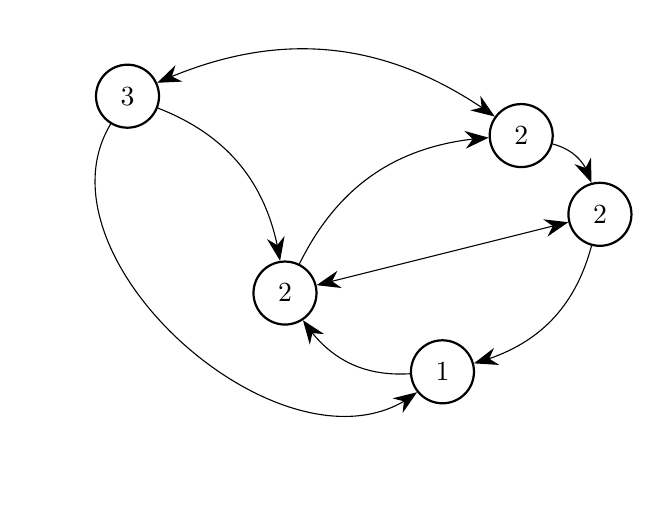
\begin{tikzpicture}[scale=1, transform shape]
    % Nodes
    \node[vertex] (A) at (0,0) {2};
    \node[vertex] (B) at (3,2) {2};
    \node[vertex] (C) at (4,1) {2};
    \node[vertex] (D) at (2,-1) {1};
    \node[vertex] (E) at (-2, 2.5) {3};

    % edges
    \draw[edge] (A) to[bend left] (B);
    \draw[edge] (B) to[bend left] (C);
    \draw[edge] (C) to[bend left] (D);
    \draw[edge] (D) to[bend left] (A);
    \draw[biedge] (A) -- (C); 
    \draw[edge] (E) to[bend right=80] (D);
    \draw[biedge] (E) to[bend left] (B);
    \draw[edge] (E) to[bend left] (A);
\end{tikzpicture}
\end{center}
\end{frame}


\subsection{Weighted}

\begin{frame}\frametitle{Weighted Graphs}
\begin{itemize}
\item In some cases we might be interested in adding a weight to each edge
\begin{itemize}
\item A cost to traverse the edge
\end{itemize}
\item It can be used in undirected or directed graphs
\end{itemize}
\begin{center}
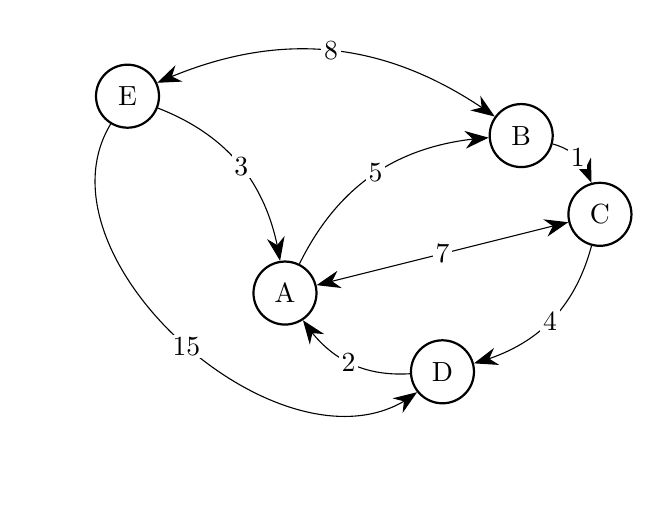
\begin{tikzpicture}[scale=1, transform shape, 
                    weight/.style={midway, fill=white, inner sep=1pt}]
    % Nodes
    \node[vertex] (A) at (0,0) {A};
    \node[vertex] (B) at (3,2) {B};
    \node[vertex] (C) at (4,1) {C};
    \node[vertex] (D) at (2,-1) {D};
    \node[vertex] (E) at (-2, 2.5) {E};

    % edges
    \draw[edge] (A) to[bend left] node[weight] {5} (B);
    \draw[edge] (B) to[bend left] node[weight] {1} (C);
    \draw[edge] (C) to[bend left] node[weight] {4} (D);
    \draw[edge] (D) to[bend left] node[weight] {2} (A);
    \draw[biedge] (A) -- node[weight] {7} (C) ; 
    \draw[edge] (E) to[bend right=80] node[weight] {15} (D);
    \draw[biedge] (E) to[bend left] node[weight] {8} (B);
    \draw[edge] (E) to[bend left] node[weight] {3} (A);
\end{tikzpicture}
\end{center}
\end{frame}

\begin{frame}\frametitle{More Terminology}
\begin{description}
\item[Path length:] Number of edges in a path
\item[Path cost:] Sum of weights in a path
\end{description}
\begin{block}{}
Calculate the path length and cost of the shortest path from E to D
\end{block}
\begin{center}
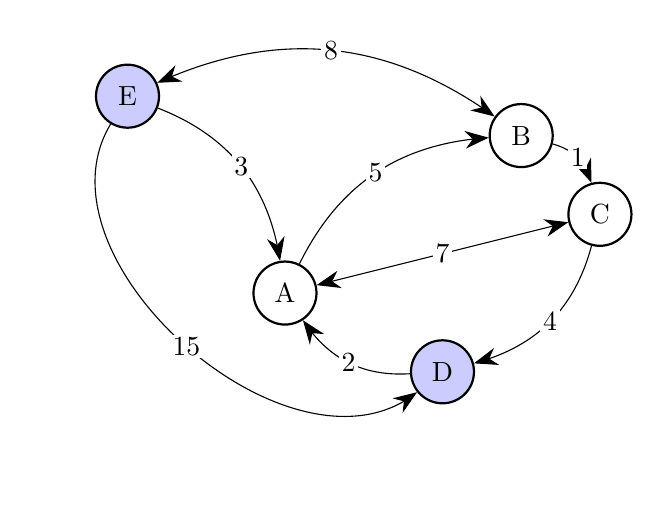
\begin{tikzpicture}[scale=1, transform shape,
                    weight/.style={midway, fill=white, inner sep=1pt}]
    % Nodes
    \node[vertex] (A) at (0,0) {A};
    \node[vertex] (B) at (3,2) {B};
    \node[vertex] (C) at (4,1) {C};
    \node[vertex, fill=blue!20] (D) at (2,-1) {D};
    \node[vertex, fill=blue!20] (E) at (-2, 2.5) {E};

    % edges
    \draw[edge] (A) to[bend left] node[weight] {5} (B);
    \draw[edge] (B) to[bend left] node[weight] {1} (C);
    \draw[edge] (C) to[bend left] node[weight] {4} (D);
    \draw[edge] (D) to[bend left] node[weight] {2} (A);
    \draw[biedge] (A) -- node[weight] {7} (C) ; 
    \draw[edge] (E) to[bend right=80] node[weight] {15} (D);
    \draw[biedge] (E) to[bend left] node[weight] {8} (B);
    \draw[edge] (E) to[bend left] node[weight] {3} (A);
\end{tikzpicture}
\end{center}
\end{frame}

\section{Graph Representation}

\begin{frame}\frametitle{From Concept to Data Structure}
\begin{itemize}
\item A graph is useful for the following questions:
    \begin{itemize}
    \item What is the shortest path between two cities?
    \item Is there a route that visits every node exactly once? 
    \item How many degrees of separation are there between two users?
    \item Are there communities or clusters of people?
    \item Which web pages are most important? (PageRank)
    \end{itemize}
\item We need a Data Structure to store graph information and work with it
\item There are different approaches
    \begin{itemize}
    \item The information on the graph (dense or sparse)
    \item The common queries (what are the edges of a vertex or does edge (u, v) exist)
    \end{itemize}
\end{itemize}
\end{frame}

\subsection{Adjacency Matrix}

\begin{frame}\frametitle{Adjacency Matrix}
\begin{itemize}
\item Use a $n\times n$ matrix where $n$ is the number of vertices
    \begin{itemize}
    \item $G[i][j] = 1$ if there is an edge from vertex i to vertex j
    \item $G[i][j] = 0$ otherwise
    \end{itemize}
\pause
\item Create the matrix for the following graph:
\end{itemize}
\begin{center}
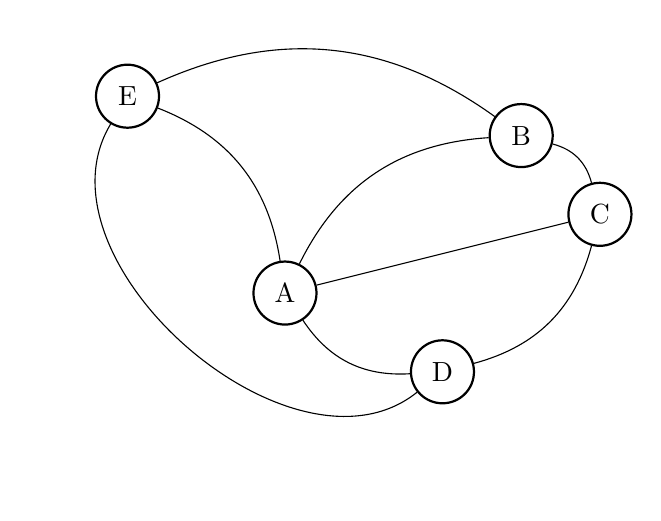
\begin{tikzpicture}[scale=1, transform shape]
    % Nodes
    \node[vertex] (A) at (0,0) {A};
    \node[vertex] (B) at (3,2) {B};
    \node[vertex] (C) at (4,1) {C};
    \node[vertex] (D) at (2,-1) {D};
    \node[vertex] (E) at (-2, 2.5) {E};

    % edges
    \draw (A) to[bend left] (B);
    \draw (B) to[bend left] (C);
    \draw (C) to[bend left] (D);
    \draw (D) to[bend left] (A);
    \draw (A) -- (C); 
    \draw (E) to[bend right=80] (D);
    \draw (E) to[bend left] (B);
    \draw (E) to[bend left] (A);
\end{tikzpicture}
\end{center}
\end{frame}

\begin{frame}\frametitle{Adjacency Matrix Undirected}
\begin{center}
$
\mathbf{G} = 
    \bordermatrix{ 
        & A & B & C & D & E \cr
      A & 0 & 1 & 1 & 1 & 1 \cr
      B & 1 & 0 & 1 & 0 & 1 \cr
      C & 1 & 1 & 0 & 1 & 0 \cr
      D & 1 & 0 & 1 & 0 & 1 \cr
      E & 1 & 1 & 0 & 1 & 0 
      }
$
\end{center}
\pause
\begin{itemize}
\item Is there any special property to this matrix? 
% diagonals 0
% symmetric
\pause
\item What happens with self edges?
\end{itemize}
\end{frame}

\begin{frame}\frametitle{Directed Adjacency Matrix}
\begin{itemize}
\item Is the adjacency matrix of this graph the same as before?
\end{itemize}
\begin{center}
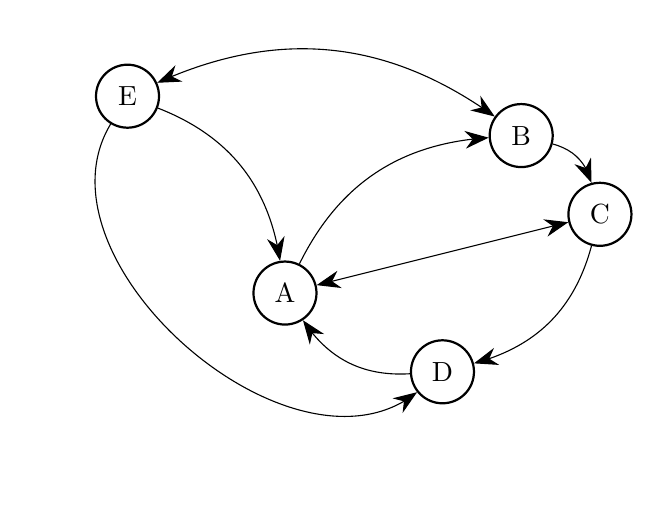
\begin{tikzpicture}[scale=1, transform shape]
    % Nodes
    \node[vertex] (A) at (0,0) {A};
    \node[vertex] (B) at (3,2) {B};
    \node[vertex] (C) at (4,1) {C};
    \node[vertex] (D) at (2,-1) {D};
    \node[vertex] (E) at (-2, 2.5) {E};

    % edges
    \draw[edge] (A) to[bend left] (B);
    \draw[edge] (B) to[bend left] (C);
    \draw[edge] (C) to[bend left] (D);
    \draw[edge] (D) to[bend left] (A);
    \draw[biedge] (A) -- (C); 
    \draw[edge] (E) to[bend right=80] (D);
    \draw[biedge] (E) to[bend left] (B);
    \draw[edge] (E) to[bend left] (A);
\end{tikzpicture}
\end{center}
\end{frame}

\begin{frame}\frametitle{Adjacency Matrix Directed}
\begin{center}
$
\mathbf{G} = 
    \bordermatrix{ 
        & A & B & C & D & E \cr
      A & 0 & 1 & 1 & 0 & 0 \cr
      B & 0 & 0 & 1 & 0 & 1 \cr
      C & 1 & 0 & 0 & 1 & 0 \cr
      D & 1 & 0 & 0 & 0 & 0 \cr
      E & 1 & 1 & 0 & 1 & 0 
      }
$
\end{center}
\pause
\begin{itemize}
\item The matrix is no longer symmetric? 
\end{itemize}
\end{frame}

\begin{frame}\frametitle{Weighted Adjacency Matrix}
\begin{itemize}
\item Now, let us work with a weighted graph.
\end{itemize}
\begin{center}
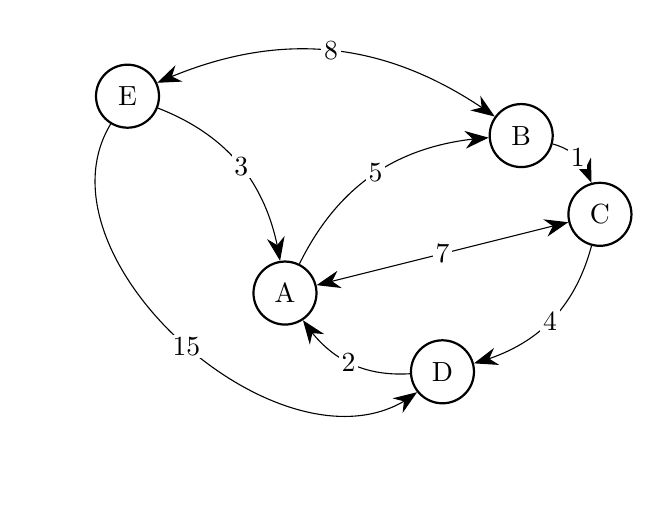
\begin{tikzpicture}[scale=1, transform shape,
                    weight/.style={midway, fill=white, inner sep=1pt}]]
    % Nodes
    \node[vertex] (A) at (0,0) {A};
    \node[vertex] (B) at (3,2) {B};
    \node[vertex] (C) at (4,1) {C};
    \node[vertex] (D) at (2,-1) {D};
    \node[vertex] (E) at (-2, 2.5) {E};

    % edges
    \draw[edge] (A) to[bend left] node[weight] {5} (B);
    \draw[edge] (B) to[bend left] node[weight] {1} (C);
    \draw[edge] (C) to[bend left] node[weight] {4} (D);
    \draw[edge] (D) to[bend left] node[weight] {2} (A);
    \draw[biedge] (A) -- node[weight] {7} (C) ; 
    \draw[edge] (E) to[bend right=80] node[weight] {15} (D);
    \draw[biedge] (E) to[bend left] node[weight] {8} (B);
    \draw[edge] (E) to[bend left] node[weight] {3} (A);
\end{tikzpicture}
\end{center}
\end{frame}

\begin{frame}\frametitle{Weighted Adjacency Matrix}
\begin{center}
$
\mathbf{G} = 
    \bordermatrix{ 
        & A & B & C & D & E \cr
      A & 0 & 5 & 7 & 0 & 0 \cr
      B & 0 & 0 & 1 & 0 & 8 \cr
      C & 7 & 0 & 0 & 4 & 0 \cr
      D & 2 & 0 & 0 & 0 & 0 \cr
      E & 3 & 8 & 0 & 15 & 0 
      }
$
\end{center}
\end{frame}

\subsection{Adjacency List}

\begin{frame}\frametitle{Adjacency List}
\begin{itemize}
\item Another option is to store a list of all adjacent vertices for each vertex.
\pause
\item Which will be the lists created for the following graph?
\end{itemize}
\begin{center}
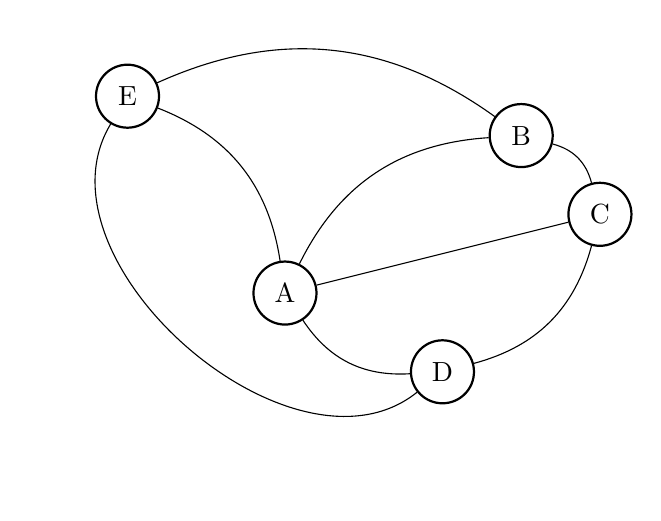
\begin{tikzpicture}[scale=1, transform shape]
    % Nodes
    \node[vertex] (A) at (0,0) {A};
    \node[vertex] (B) at (3,2) {B};
    \node[vertex] (C) at (4,1) {C};
    \node[vertex] (D) at (2,-1) {D};
    \node[vertex] (E) at (-2, 2.5) {E};

    % edges
    \draw (A) to[bend left] (B);
    \draw (B) to[bend left] (C);
    \draw (C) to[bend left] (D);
    \draw (D) to[bend left] (A);
    \draw (A) -- (C); 
    \draw (E) to[bend right=80] (D);
    \draw (E) to[bend left] (B);
    \draw (E) to[bend left] (A);
\end{tikzpicture}
\end{center}
\end{frame}


\begin{frame}\frametitle{Adjacency List Example}
\begin{description}
\item[A:] B, C, D, E
\item[B:] A, C, E
\item[C:] A, B, D
\item[D:] A, C, E
\item[E:] A, B, D
\end{description}
\end{frame}

\begin{frame}[fragile]\frametitle{Adjacency List on Python}
\begin{itemize}
\item What is the best structure for the Adjacency List on Python?
% Dictionary or class
\pause
\item We can use a dictionary
\begin{lstlisting}
G = {'A': ['B', 'C', 'D', 'E'], 
     'B': ['A', 'C', 'E'],
     ...}
\end{lstlisting}
\pause
\item Or we can use something similar to the trees
\begin{lstlisting}
class Vertex:
    def __init__(self, id):
        self.__id = id
        self.__adjacent = []
\end{lstlisting}
\end{itemize}
\end{frame}

\begin{frame}\frametitle{Including More Information}
\begin{itemize}
\item What modifications are necessary to differentiate an undirected from a directed graph?
\item What happens if the graph is weighted?
\end{itemize}
\end{frame}

\subsection{Which One to Choose}

\begin{frame}\frametitle{Complexity}
\begin{center}
\begin{tabular}{@{} lll @{}}
\toprule
\textbf{Operation} & \textbf{Adjacency Matrix} & \textbf{Adjacency List} \\
\midrule
Space Complexity                 & $O(|V|^2)$           & $O(|V| + |E|)$            \\
Add an edge                      & $O(1)$               & $O(1)$                \\
Remove an edge                   & $O(1)$               & $O(\deg(v))$          \\
Check if edge $(u,v)$ exists     & $O(1)$               & $O(\deg(v))$          \\
Enumerate all neighbours         & $O(|V|)$             & $O(\deg(v))$          \\
Enumerate all edges              & $O(|V|^2)$           & $O(|V| + |E|)$            \\
Edge weight retrieval            & $O(1)$               & $O(\deg(v))$          \\
DFS/BFS traversal                & $O(|V|^2)$           & $O(|V| + |E|)$            \\
\bottomrule
\end{tabular}
\end{center}
\end{frame}

\begin{frame}\frametitle{Memory Usage}
\begin{itemize}
\item Adjacency matrix
    \begin{itemize}
    \item Always $|V|^2$ space (can be reduced if undirected)
    \item Good for dense graphs where $|E| \sim |V|^2$
    \end{itemize}
\item Adjacency list
    \begin{itemize}
    \item Space proportional to $|V| + |E|$
    \item Best for sparse graphs where $|E| \ll |V|^2$
    \end{itemize}
\end{itemize}
\end{frame}

\begin{frame}\frametitle{Use Cases}
\centering
\begin{tabular}{@{} p{0.6\textwidth} l @{}}
\toprule
\textbf{Use Case} & \textbf{Best Representation} \\
\midrule
Graph is dense & Adjacency Matrix \\
Graph is sparse & Adjacency List \\
Frequently check edge existence & Adjacency Matrix \\
Iterate over neighbours often & Adjacency List \\
Want to minimize space usage & Adjacency List \\
Using Dijkstra's algorithm & Adjacency List \\
Using Floyd-Warshall algorithm & Adjacency Matrix \\
\bottomrule
\end{tabular}
\end{frame}

\section{Exercises}

% Ejercicio para crear lista de caminos posibles y su coste total
% Se puede asemejar a la creacion de un arbol donde cada nodo tendra como hijos los posibles caminos
% para evitar ciclos no se puede añadir como hijo si ya esta en algun punto hacia la raiz
\begin{frame}\frametitle{Find Paths}
\begin{enumerate}
\item Find the shortest path from B to H
\item Find the shortest path from D to G
\item Can we automate it?
\end{enumerate}
\begin{center}
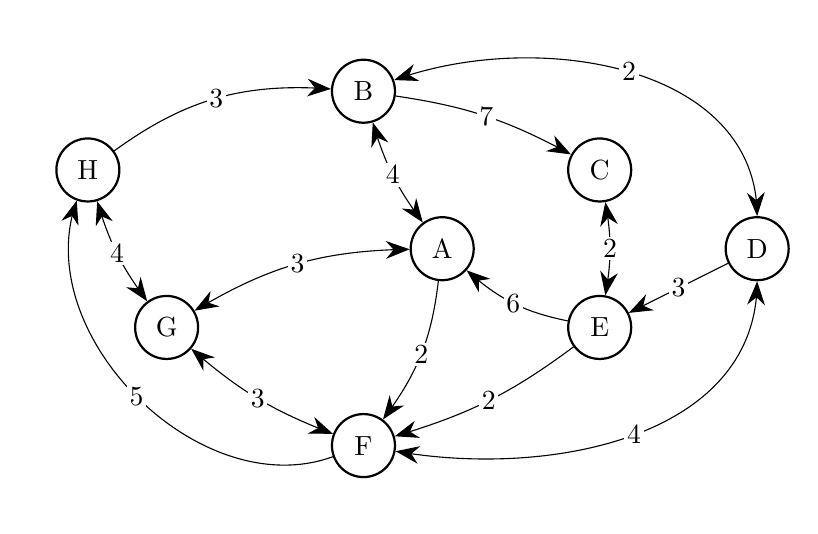
\begin{tikzpicture}

% Nodes with randomized positions
\node[vertex] (A) at (3,1)     {A};
\node[vertex] (B) at (2,3)     {B};
\node[vertex] (C) at (5,2)     {C};
\node[vertex] (D) at (7,1)     {D};
\node[vertex] (E) at (5,0)     {E};
\node[vertex] (F) at (2,-1.5)    {F};
\node[vertex] (G) at (-0.5,0)    {G};
\node[vertex] (H) at (-1.5,2)    {H};

% Directed edges with weights (max 3 out/in edges per node)
\draw[biedge] (A) to[bend left=10] node[weight] {4} (B);
\draw[biedge] (A) to[bend right=15] node[weight] {3} (G);
\draw[edge] (A) to[bend left=15] node[weight] {2} (F);

\draw[edge] (B) to[bend left=10] node[weight] {7} (C);
\draw[biedge] (B) to[out=20, in=90] node[weight] {2} (D);

\draw[biedge] (C) to[bend left=10] node[weight] {2} (E);

\draw[edge] (D) to node[weight] {3} (E);
\draw[biedge] (D) to[out=-90, in=-10] node[weight] {4} (F);

\draw[edge] (E) to[bend left=15] node[weight] {6} (A);
\draw[edge] (E) to[bend left=10] node[weight] {2} (F);

\draw[biedge] (F) to[bend left=10] node[weight] {3} (G);
\draw[edge] (F) to[out=200, in=-110] node[weight] {5} (H);

\draw[biedge] (G) to[bend left=10] node[weight] {4} (H);

\draw[edge] (H) to[bend left=20] node[weight] {3} (B);
\end{tikzpicture}
\end{center}
\end{frame}

\end{document}






